%%%%%%%%%%%%%%%%%%%%%%%%%%%%%%%%%%%%%%%%%%%%%%%%%%%%%%%%%%%%%%%%%%%%%%%%%%%%%%%%
% Thesis / Project Report
% LaTeX Template
% Version 2.0 (08/04/16)
%
% Author:
% Siddhant Shrivastava
% https://github.com/sidcode/bits-pilani-thesis-template-latex
%
% This template is heavily based on the work of Darshit Shah, Steven Gunn and Sunil Patel
% Darshit Shah
% https://github.com/darnir/BPHC-LaTeX-Report-Class
% Steven Gunn
% http://users.ecs.soton.ac.uk/srg/softwaretools/document/templates/
% and
% Sunil Patel
% http://www.sunilpatel.co.uk/thesis-template/
%
% License:
% CC BY-NC-SA 4.0 (http://creativecommons.org/licenses/by-nc-sa/4.0/)
%
% Note:
% Make sure to edit document variables in the Thesis.cls file
%
%%%%%%%%%%%%%%%%%%%%%%%%%%%%%%%%%%%%%%%%%%%%%%%%%%%%%%%%%%%%%%%%%%%%%%%%%%%%%%%%

%-------------------------------------------------------------------------------
%	PACKAGES AND OTHER DOCUMENT CONFIGURATIONS
%-------------------------------------------------------------------------------

\documentclass[11pt, a4paper, oneside]{Thesis} % Paper size, default font size
                                               % and one-sided paper

\graphicspath{{Pictures/}} % Specifies the directory where pictures are stored

\usepackage[backend=bibtex]{biblatex}
\bibliography{Bibliography.bib}

\title{\ttitle} % Defines the thesis title - don't touch this

\begin{document}

\frontmatter % Use roman numbering style (i, ii...) for the pre-content pages

\setstretch{1.3} % Line spacing of 1.3

% Define page headers using FancyHdr package and set up for one-sided printing
\fancyhead{} % Clears all page headers and footers
\rhead{\thepage} % Sets the right side header to show the page number
\lhead{} % Clears the left side page header

\pagestyle{fancy} % Finally, use the "fancy" page style to implement the
                  %FancyHdr headers

% Input all the variables used in the document. Please fill out the
% variables.tex file with all your details.
%-------------------------------------------------------------------------------
%	DOCUMENT VARIABLES
%
%	Fill in the lines below to set the various variables for the document
%-------------------------------------------------------------------------------

%-------------------------------------------------------------------------------
% Your thesis title - this is used in the title and abstract
% Command: \ttitle
\thesistitle{Highjacking the Rust programming language for high performant in-situ analytics}
%-------------------------------------------------------------------------------
% The document type: Thesis / report, etc.
% Command: \doctype
\documenttype{Undergraduate Thesis}
%-------------------------------------------------------------------------------
% Your supervisor's name - this is used in the title page
% Command: \supname
\supervisor{Dr. Bruno \textsc{RAFFIN}}
%-------------------------------------------------------------------------------
% The supervisor's position - Used on Certificate
% Command: \suppos
\supervisorposition{Director of Reserch}
%-------------------------------------------------------------------------------
% Supervisor's institute
% Command: \supinst
\supervisorinstitute{INRIA Grenoble Rhone-Alpes}
%%-------------------------------------------------------------------------------
%% Your supervisor's name - this is used in the title page
%% Command: \supname
%\supervisor{Dr. Frederic \textsc{WAGNER}}
%%-------------------------------------------------------------------------------
%% The supervisor's position - Used on Certificate
%% Command: \suppos
%\supervisorposition{Associate Professor}
%%-------------------------------------------------------------------------------
%% Supervisor's institute
%% Command: \supinst
%\supervisorinstitute{ENSIMAG, Grenoble}
%-------------------------------------------------------------------------------
% Your Co-Supervisor's name
% Command: \cosupname
\cosupervisor{Prof. Sundar Shan \textsc{Balasubramaniam}}
%-------------------------------------------------------------------------------
% Co-Supervisor's Position - Used on Certificate
% Command: \cosuppos
\cosupervisorposition{Professor}
%-------------------------------------------------------------------------------
% Co-Supervisor's Institute
% Command: \cosupinst
\cosupervisorinstitute{BITS-Pilani Pilani Campus}
%-------------------------------------------------------------------------------
% Your Examiner's name. Not currently used anywhere.
% Command: \examname
\examiner{}
%-------------------------------------------------------------------------------
% Name of your degree
% Command: \degreename
\degree{Bachelor of Engineering (Hons.)}
%-------------------------------------------------------------------------------
% The BITS Course Code for which this report is written
% COmmand: \ccode
\coursecode{BITS F421T}
%-------------------------------------------------------------------------------
% The name of the Course
% Command: \cname
\coursename{Thesis}
%-------------------------------------------------------------------------------
% Your name. Extend manually in case of multiple authors
% Command: \authornames
\authors{Saurabh Manish \textsc{Raje}}
%-------------------------------------------------------------------------------
% Your ID Number - used on the Title page and abstract
% Command: \idnum
\IDNumber{2015A7TS0045P}
%-------------------------------------------------------------------------------
% Your address
% Command: \addressnames
\addresses{}
%-------------------------------------------------------------------------------
% Your subject area
% Command: \subjectname
\subject{}
%-------------------------------------------------------------------------------
% Keywords for this report.
% Command: \keywordnames
\keywords{}
%-------------------------------------------------------------------------------
% University details
% Command: \univname
\university{\texorpdfstring{\href{http://www.bits-pilani.ac.in/} % URL
                {Birla Institute of Technology and Science Pilani}} % University name
                {Birla Institute of Technology and Science Pilani}}
%-------------------------------------------------------------------------------
% University details, in Capitals
% Command: \UNIVNAME
\UNIVERSITY{\texorpdfstring{\href{http://www.bits-pilani.ac.in/} % URL
                {BIRLA INSTITUTE OF TECHNOLOGY AND SCIENCE PILANI}} % name in capitals
                {BIRLA INSTITUTE OF TECHNOLOGY AND SCIENCE PILANI}}

%-------------------------------------------------------------------------------
% Campus Name
% Command: \campusname
\campus{Pilani Campus}

%-------------------------------------------------------------------------------
% Campus Name, in capitals
% Command: \CAMPUSNAME
\CAMPUS{PILANI CAMPUS}


%-------------------------------------------------------------------------------
% Department Details
% Command: \deptname
\department{\texorpdfstring{\href{http://www.bits-pilani.ac.in/pilani/computerscience/ComputerScience} % Your department's URL
                {Computer Science \& Information Systems}} % Your department's name
                {Computer Science}}
%-------------------------------------------------------------------------------
% Department details, in Capitals
% Command: \DEPTNAME
\DEPARTMENT{\texorpdfstring{\href{http://www.bits-pilani.ac.in/pilani/computerscience/ComputerScience} % Your department's URL
                {COMPUTER SCIENCE \& INFORMATION SYSTEMS}} % Your department's name in capitals
                {COMPUTER SCIENCE \& INFORMATION SYSTEMS}}
%-------------------------------------------------------------------------------
% Research Group Details
% Command: \groupname
\group{\texorpdfstring{\href{Research Group Web Site URL Here (include http://)}
                {Research Group Name}} % Your research group's name
                {Research Group Name}}
%-------------------------------------------------------------------------------
% Research Group Details, in Capitals
% Command: \GROUPNAME
\GROUP{\texorpdfstring{\href{Research Group Web Site URL Here (include http://)}
                {RESEARCH GROUP NAME (IN BLOCK CAPITALS)}}
                {RESEARCH GROUP NAME (IN BLOCK CAPITALS)}}
%-------------------------------------------------------------------------------
% Faculty details
% Command: \facname
\faculty{\texorpdfstring{\href{Faculty Web Site URL Here (include http://)}
                {Faculty Name}}
                {Faculty Name}}
%-------------------------------------------------------------------------------
% Faculty details, in Capitals
% Command: \FACNAME
\FACULTY{\texorpdfstring{\href{Faculty Web Site URL Here (include http://)}
                {FACULTY NAME (IN BLOCK CAPITALS)}}
                {FACULTY NAME (IN BLOCK CAPITALS)}}
%-------------------------------------------------------------------------------


%-------------------------------------------------------------------------------
%   NON-CONTENT PAGES
%-------------------------------------------------------------------------------
\maketitle
\Declaration
\Certificate
%\Quotation{Insert random Quote here. Publish like a boss.}{Your Name}

\begin{abstract}
\ldots
\end{abstract}

\begin{acknowledgements}
The acknowledg and the people to thank go here, don't forget to include
your project advisor\ldots
\end{acknowledgements}

%-------------------------------------------------------------------------------
%	LIST OF CONTENTS/FIGURES/TABLES PAGES
%-------------------------------------------------------------------------------

% The page style headers have been "empty" all this time, now use the "fancy"
% headers as defined before to bring them back
\pagestyle{fancy}

\lhead{\emph{Contents}} % Set the left side page header to "Contents"
\tableofcontents % Write out the Table of Contents

% Set the left side page header to "List of Figures"
\lhead{\emph{List of Figures}}
\listoffigures % Write out the List of Figures

 % Set the left side page header to "List of Tables"
\lhead{\emph{List of Tables}}
\listoftables % Write out the List of Tables

%-------------------------------------------------------------------------------
%	ABBREVIATIONS
%-------------------------------------------------------------------------------

\clearpage % Start a new page

 % Set the line spacing to 1.5, this makes the following tables easier to read
\setstretch{1.5}

\lhead{\emph{Abbreviations}} % Set the left side page header to "Abbreviations"
\listofsymbols{ll} % Include a list of Abbreviations (a table of two columns)
{
\textbf{LAH} & \textbf{L}ist \textbf{A}bbreviations \textbf{H}ere \\
%\textbf{Acronym} & \textbf{W}hat (it) \textbf{S}tands \textbf{F}or \\
}

%-------------------------------------------------------------------------------
%	PHYSICAL CONSTANTS/OTHER DEFINITIONS
%-------------------------------------------------------------------------------

%\clearpage % Start a new page

% Set the left side page header to "Physical Constants"
%\lhead{\emph{Physical Constants}}

 % Include a list of Physical Constants (a four column table)
%\listofconstants{lrcl}
%{
%Speed of Light & $c$ & $=$ & $2.997\ 924\ 58\times10^{8}\ \mbox{ms}^{-\mbox{s}}$ (exact)\\
%% Constant Name & Symbol & = & Constant Value (with units) \\
%}

%-------------------------------------------------------------------------------
%	SYMBOLS
%-------------------------------------------------------------------------------

%\clearpage % Start a new page
%
%\lhead{\emph{Glossary}} % Set the left side page header to "Symbols"
%
%\listofnomenclature % List the nomenclature. (We use the glossaries package)

%-------------------------------------------------------------------------------
%	DEDICATION
%-------------------------------------------------------------------------------

%\setstretch{1.3} % Return the line spacing back to 1.3
%
%\pagestyle{empty} % Page style needs to be empty for this page
%
%% Dedication text
%%\Dedicatory{Dedicate this to someone, anyone.}
%
%\addtocontents{toc}{\vspace{2em}} % Add a gap in the Contents, for aesthetics

%-------------------------------------------------------------------------------
%	THESIS CONTENT - CHAPTERS
%-------------------------------------------------------------------------------

\mainmatter % Begin numeric (1,2,3...) page numbering

\pagestyle{fancy} % Return the page headers back to the "fancy" style

% Include the chapters of the thesis as separate files from the Chapters folder
% Uncomment the lines as you write the chapters

% Chapter 1

\chapter{The Rust programming language} % Main chapter title

\label{Chapter1} % For referencing the chapter elsewhere, use \ref{Chapter1}

\lhead{Chapter 1. \emph{About Rust}} % This is for the header on each page - perhaps a shortened title

%----------------------------------------------------------------------------------------

\section{The need for Rust}
While modern day languages provide higher amounts of abstraction and ease of programming, they either come at the cost of safety, or runtime performance, or both. Systems development is still dominated by C/C++ due to the high performance that they offer. However, it is extremely easy to create fundamental loopholes in huge systems that may lead to invalid memory access and crash the entire system, if the programmer is lucky. In the worst case, there may be data corruption due to an invalid access that is extremely hard to trace.

Rust addresses the dire need for a fast and safe systems development language. It goes above and beyond in this regard to offer zero cost abstractions in the form of abstract traits and types that allow seamless integration of new features with an existing system. Furthermore, it also allows for functional programming with its lazy iterators API. This generates highly optimized machine code with performance comparable to C.

Compilable code written in Rust can never lead to data races, dangling pointers, double frees or memory leaks. This comes from a simple sacrifice of the mutable state. By imposing the invariant that each memory location must have a single mutable reference to it (that can not overlap in time with an immutable reference), all above problems are prevented. Furthermore, it allows the language to offer automated memory management at minimal overhead as opposed to traditional methods of garbage collection.
%----------------------------------------------------------------------------------------

\section{Some quirks of programming in Rust}

The invariant of not having multiple mutable references to a memory object severely restricts syntactic expression of any given algorithm. The language hence suffers from a steep initial learning curve. The further sections shall elaborate some jargon that describes the memory model.

\subsection{Ownership}
The concept of ownership imposes the following rules[Cite the book here]:
\begin{itemize}
\item Each value in Rust has a variable that is its \emph{owner}.
\item This owner has mutable access to the value/memory object in question.
\item There can be only one owner at a given time (read: scope).
\item When the owner goes out of scope, the value is dropped.
\end{itemize}
Here it is important to note that all the analysis regarding ownership is carried out at compile time, and hence calls to drop objects are inserted by the compiler. This therefore provides memory safety and management at minimal runtime overhead.

\subsection{Movement and copy}
When variables are reassigned or passed around across functions, they adopt exactly one of two semantics, move and copy. Typically, any variable on the heap adopts the former while lightweight datatypes residing on the stack adopt the latter.

The move semantic changes the owner of the variable. This means that the scope of the variable is now the scope of it's new owner. The previous owner is an invalid reference to the variable, and the compiler would trigger compile-time errors for any attempt to use the previous owner.

The copy semantic on the other hand creates a deep copy of the data contained in the variable. We now have two different variables at separate locations in the memory, and having separate owners. The data that they contain, however, is the same.


\subsection{Borrows and lifetimes}
The former design requires unnecessary moves for situations (for example in case a function intends to read some data, it must be moved in and out). As an alternative, the language offers it's own notion of references. When a reference is created to any variable, it is called a borrow of that variable. Each reference has a lifetime that defines how long the reference is usable. This lifetime can never be more than that of the data referred to. Again, these checks are carried out at compile time. By a way of default, all references are immutable. However, by explicitly obtaining the reference with the \emph{'\&mut'} specifier, it is possible to get a mutable reference. As shown in Figure \ref{fig:borrow_checker}, the compiler throws a compiler time error if an immutable reference and a mutable reference are held on the same object.

\begin{figure}%[opt-rat]
	%\centering
    \includegraphics[scale=0.25]{Pictures/borrow_checker.jpg}
		%\rule{35em}{0.5pt}
    \caption[Optimization]{The "borrow checker" in the compiler guarding against lost updates.}
	\label{fig:borrow_checker}
\end{figure}
Furthermore, the compiler imposes a check to ensure that the lifetimes of two mutable references, (or that of one mutable reference with an immutable reference) do(es) not overlap.

\subsection{Generic types and traits}
The language offers powerful abstractions in the form of generic types and \emph{traits}. A \emph{trait} is essentially a set of functions (and possibly some types as well). Typically, one or more functions in the trait are not implemented. They have a particular signature to be followed as is. However, one or many functions can be defined and implemented in the trait. In such a case, after implementing just the abstract functions, the programmer has the rest of the functions of the trait at his disposal without having to implement them. The best example of this is the \textbf{Iterator} trait. After providing the implementation of the \textbf{next()} method, the entire functional API is available for use on the given iterator. This feature is analogous to interfaces in Java, for example. Traits can be extended from each other in order to create an object oriented hierarchy.

This dovetails with the notion of a generic type. Rust offers the possibility of using generic types in trait or function definition. A generic type is constrained by certain trait implementations. This essentially means that the signature is valid for any and all types that implement the given trait(s). This is extremely useful since any future types being introduced in the system would automatically have various functionalities supported with a few trait implementations. Consider the following example:

\begin{verbatim}
fn largest<T: PartialOrd + Copy>(list: &[T]) -> T {
    let mut largest = list[0];
    for &item in list.iter() {
        if item > largest {
            largest = item;
        }
    }
    largest
}
\end{verbatim}

This function uses a generic type \textbf{T} and describes how to find the "\emph{largest}" element out of a list of elements of type \textbf{T} (it will borrow this list). The type \textbf{T} is generic in that it can be anything that implements ParitalOrd and Copy traits.

% Chapter 1

\chapter{Concurrency in Rust} % Main chapter title

\label{Chapter2} % For referencing the chapter elsewhere, use \ref{Chapter2}

\lhead{Chapter 2. \emph{Concurrency in Rust}} % This is for the header on each page - perhaps a shortened title

%----------------------------------------------------------------------------------------

\section{The Thread API}
The Rust language provides a basic thread API that contains primitives \emph{spawn} and \emph{join}. \emph{Spawn} creates a thread and passes it a closure - that it took in - as an argument. The \emph{join} on the other hand forces the calling thread to wait on a given \emph{JoinHandle} that was created by a spawned thread. Furthermore, it also offers synchronization primititves such as Mutexes, Condition Variables, Barriers and Reader Writer Locks.

\section{Rayon}

There is a more abstract (functional) alternative for shared memory parallelism called the \textbf{Rayon API}. As far as the programmer is concerned, a sequential functional code can be parallelized with nearly no additional effort. Internally, Rayon uses recursive task splitting to balance load across threads.

Specifically, it provides a parallel iterator on which various operations (same as in the sequential domain) can be performed one after the other, forming a pipeline. Internally,
\begin{itemize}
    \item This iterator is split recursively into two halves until the balanced binary tree (of splits) reaches a specific depth.
    \item Each split is a task that is pushed on the stack.
    \item In case there are any idle threads, they steal a task from this stack.
    \item The stealer continues the above procedure, with the depth measure reset to 1.
\end{itemize}
%[ADD A RAYON LOG HERE]
Below is an example of a code that uses the Rayon API to parallelize the sum of a list of numbers.
\begin{verbatim}
extern crate rayon
use rayon::prelude::*;
fn main() {
    let inp = vec![1, 2, 3, 4, 5, 6, 7];
    println!("{}",inp.par_iter().fold_with(0, |acc, x| acc + x).sum::<u32>());
}
\end{verbatim}
%----------------------------------------------------------------------------------------
%\section{An alternative to Rayon}
%In the context of high performance computing, the abstraction provided by Rayon currently comes at a high cost of task creation overhead. This is because the heuristic for splitting is far from perfect. As described in the previous section, Rayon splits tasks only till a specific depth is reached. This also implies that if the depth has been reached by all threads, but there is somehow an idle thread in the system, there would be no task splitting and hence that thread would remain idle forever.
%
%Furthermore, this problem compounds in the case of nested parallel iterators, wherein Rayon would not differentiate between the tasks created by these levels. It would hence push these on a common stack for a thread. A steal operation would therefore retrieve a task from the lowermost hierarchy while there exist tasks at a higher hierarchy.
%
%In conclusion, the programmer would hence pay for an extremely high task creation overhead, while the load distribution would be more skewed towards the threads that started first.
%
%This motivates the design and implementation of an Adaptive API developed in-house at INRIA.
%
%\subsection{The adaptive task splitting algorithm}
%
%If you are new to \LaTeX{}, there is a very good eBook -- freely available online as a PDF file -- called, ``The Not So Short Introduction to \LaTeX{}''. The book's title is typically shortened to just ``lshort''. You can download the latest version (as it is occasionally updated) from here:\\
%\href{http://www.ctan.org/tex-archive/info/lshort/english/lshort.pdf}{\texttt{http://www.ctan.org/tex-archive/info/lshort/english/lshort.pdf}}
%
%It is also available in several other languages. Find yours from the list on this page:\\
%\href{http://www.ctan.org/tex-archive/info/lshort/}{\texttt{http://www.ctan.org/tex-archive/info/lshort/}}
%
%It is recommended to take a little time out to learn how to use \LaTeX{} by creating several, small `test' documents. Making the effort now means you're not stuck learning the system when what you \emph{really} need to be doing is writing your thesis.
%
%\subsection{Handling nested parallelism}
%
%If you are writing a technical or mathematical thesis, then you may want to read the document by the AMS (American Mathematical Society) called, ``A Short Math Guide for \LaTeX{}''. It can be found online here:\\
%\href{http://www.ams.org/tex/amslatex.html}{\texttt{http://www.ams.org/tex/amslatex.html}}\\
%under the ``Additional Documentation'' section towards the bottom of the page.

% Chapter 1

\chapter{Chapter Title Here} % Main chapter title

\label{Chapter3} % For referencing the chapter elsewhere, use \ref{Chapter1} 

\lhead{Chapter 1. \emph{Chapter Title Here}} % This is for the header on each page - perhaps a shortened title

%----------------------------------------------------------------------------------------

\section{elcome and Thank You}
Welcome to this \LaTeX{} Thesis Template, a beautiful and easy to use template for writing a thesis using the \LaTeX{} typesetting system.

If you are writing a thesis (or will be in the future) and its subject is technical or mathematical (though it doesn't have to be), then creating it in \LaTeX{} is highly recommended as a way to make sure you can just get down to the essential writing without having to worry over formatting or wasting time arguing with your word processor.

\LaTeX{} is easily able to professionally typeset documents that run to hundreds or thousands of pages long. With simple mark-up commands, it automatically sets out the table of contents, margins, page headers and footers and keeps the formatting consistent and beautiful. One of its main strengths is the way it can easily typeset mathematics, even \emph{heavy} mathematics. Even if those equations are the most horribly twisted and most difficult mathematical problems that can only be solved on a super-computer, you can at least count on \LaTeX{} to make them look stunning.

%----------------------------------------------------------------------------------------

\section{Learning \LaTeX{}}

\LaTeX{} is not a WYSIWYG (What You See is What You Get) program, unlike word processors such as Microsoft Word or Apple's Pages. Instead, a document written for \LaTeX{} is actually a simple, plain text file that contains \emph{no formatting}. You tell \LaTeX{} how you want the formatting in the finished document by writing in simple commands amongst the text, for example, if I want to use \textit{italic text for emphasis}, I write the `$\backslash$\texttt{textit}\{\}' command and put the text I want in italics in between the curly braces. This means that \LaTeX{} is a ``mark-up'' language, very much like HTML.

\subsection{A (not so short) Introduction to \LaTeX{}}

If you are new to \LaTeX{}, there is a very good eBook -- freely available online as a PDF file -- called, ``The Not So Short Introduction to \LaTeX{}''. The book's title is typically shortened to just ``lshort''. You can download the latest version (as it is occasionally updated) from here:\\
\href{http://www.ctan.org/tex-archive/info/lshort/english/lshort.pdf}{\texttt{http://www.ctan.org/tex-archive/info/lshort/english/lshort.pdf}}

It is also available in several other languages. Find yours from the list on this page:\\
\href{http://www.ctan.org/tex-archive/info/lshort/}{\texttt{http://www.ctan.org/tex-archive/info/lshort/}}

It is recommended to take a little time out to learn how to use \LaTeX{} by creating several, small `test' documents. Making the effort now means you're not stuck learning the system when what you \emph{really} need to be doing is writing your thesis.

\subsection{A Short Math Guide for \LaTeX{}}

If you are writing a technical or mathematical thesis, then you may want to read the document by the AMS (American Mathematical Society) called, ``A Short Math Guide for \LaTeX{}''. It can be found online here:\\
\href{http://www.ams.org/tex/amslatex.html}{\texttt{http://www.ams.org/tex/amslatex.html}}\\
under the ``Additional Documentation'' section towards the bottom of the page.

\subsection{Common \LaTeX{} Math Symbols}
There are a multitude of mathematical symbols available for \LaTeX{} and it would take a great effort to learn the commands for them all. The most common ones you are likely to use are shown on this page:\\
\href{http://www.sunilpatel.co.uk/latexsymbols.html}{\texttt{http://www.sunilpatel.co.uk/latexsymbols.html}}

You can use this page as a reference or crib sheet, the symbols are rendered as large, high quality images so you can quickly find the \LaTeX{} command for the symbol you need.

\subsection{\LaTeX{} on a Mac}
 
The \LaTeX{} package is available for many systems including Windows, Linux and Mac OS X. The package for OS X is called MacTeX and it contains all the applications you need -- bundled together and pre-customised -- for a fully working \LaTeX{} environment and workflow.
 
MacTeX includes a dedicated \LaTeX{} IDE (Integrated Development Environment) called ``TeXShop'' for writing your `\texttt{.tex}' files and ``BibDesk'': a program to manage your references and create your bibliography section just as easily as managing songs and creating playlists in iTunes.

%----------------------------------------------------------------------------------------

\section{Getting Started with this Template}

If you are familiar with \LaTeX{}, then you can familiarise yourself with the contents of the Zip file and the directory structure and then place your own information into the `\texttt{Thesis.cls}' file. Section \ref{FillingFile} on page \pageref{FillingFile} tells you how to do this. Make sure you read section \ref{ThesisConventions} about thesis conventions to get the most out of this template and then get started with the `\texttt{Thesis.tex}' file straightaway.

If you are new to \LaTeX{} it is recommended that you carry on reading through the rest of the information in this document.

\subsection{About this Template}

This \LaTeX{} Thesis Template is originally based and created around a \LaTeX{} style file created by Steve R.\ Gunn from the University of Southampton (UK), department of Electronics and Computer Science. You can find his original thesis style file at his site, here:\\
\href{http://www.ecs.soton.ac.uk/~srg/softwaretools/document/templates/}{\texttt{http://www.ecs.soton.ac.uk/$\sim$srg/softwaretools/document/templates/}}

My thesis originally used the `\texttt{ecsthesis.cls}' from his list of styles. However, I knew \LaTeX{} could still format better. To get the look I wanted, I modified his style and also created a skeleton framework and folder structure to place the thesis files in.

This Thesis Template consists of that modified style, the framework and the folder structure. All the work that has gone into the preparation and groundwork means that all you have to bother about is the writing.

Before you begin using this template you should ensure that its style complies with the thesis style guidelines imposed by your institution. In most cases this template style and layout will be suitable. If it is not, it may only require a small change to bring the template in line with your institution's recommendations.

%----------------------------------------------------------------------------------------

\section{What this Template Includes}

\subsection{Folders}

This template comes as a single Zip file that expands out to many files and folders. The folder names are mostly self-explanatory:

\textbf{Appendices} -- this is the folder where you put the appendices. Each appendix should go into its own separate `\texttt{.tex}' file. A template is included in the directory.

\textbf{Chapters} -- this is the folder where you put the thesis chapters. A thesis usually has about seven chapters, though there is no hard rule on this. Each chapter should go in its own separate `\texttt{.tex}' file and they usually are split as:
\begin{itemize}
\item Chapter 1: Introduction to the thesis topic
\item Chapter 2: Background information and theory
\item Chapter 3: (Laboratory) experimental setup
\item Chapter 4: Details of experiment 1
\item Chapter 5: Details of experiment 2
\item Chapter 6: Discussion of the experimental results
\item Chapter 7: Conclusion and future directions
\end{itemize}
This chapter layout is specialised for the experimental sciences.

\textbf{Figures} -- this folder contains all figures for the thesis. These are the final images that will go into the thesis document.

\textbf{Primitives} -- this is the folder that contains scraps, particularly because one final image in the `Figures' folder may be made from many separate images and photos, these source images go here. This keeps the intermediate files separate from the final thesis figures.

\subsection{Files}

Included are also several files, most of them are plain text and you can see their contents in a text editor. Luckily, many of them are auxiliary files created by \LaTeX{} or BibTeX and which you don't need to bother about:

\textbf{Bibliography.bib} -- this is an important file that contains all the bibliographic information and references that you will be citing in the thesis for use with BibTeX. You can write it manually, but there are reference manager programs available that will create and manage it for you. Bibliographies in \LaTeX{} are a large subject and you may need to read about BibTeX before starting with this.

\textbf{Thesis.cls} -- this is an important file. It is the style file that tells \LaTeX{} how to format the thesis. You will also need to open this file in a text editor and fill in your own information (such as name, department, institution). Luckily, this is not too difficult and is explained in section \ref{FillingFile} on page \pageref{FillingFile}.

\textbf{Thesis.pdf} -- this is your beautifully typeset thesis (in the PDF file format) created by \LaTeX{}.

\textbf{Thesis.tex} -- this is an important file. This is the file that you tell \LaTeX{} to compile to produce your thesis as a PDF file. It contains the framework and constructs that tell \LaTeX{} how to layout the thesis. It is heavily commented so you can read exactly what each line of code does and why it is there. After you put your own information into the `\texttt{Thesis.cls}' file, go to this file and begin filling it in -- you have now started your thesis!

\textbf{vector.sty} -- this is a \LaTeX{} package, it tells \LaTeX{} how to typeset mathematical vectors. Using this package is very easy and you can read the documentation on the site (you just need to look at the `\texttt{vector.pdf}' file):\\
\href{http://www.ctan.org/tex-archive/macros/latex/contrib/vector/}{\texttt{http://www.ctan.org/tex-archive/macros/latex/contrib/vector/}}

\textbf{lstpatch.sty} -- this is a \LaTeX{} package required by this LaTeX template and is included as not all \TeX{} distributions have it installed by default. You do not need to modify this file.

Files that are \emph{not} included, but are created by \LaTeX{} as auxiliary files include:

\textbf{Thesis.aux} -- this is an auxiliary file generated by \LaTeX{}, if it is deleted \LaTeX{} simply regenerates it when you run the main `\texttt{.tex}' file.

\textbf{Thesis.bbl} -- this is an auxiliary file generated by BibTeX, if it is deleted, BibTeX simply regenerates it when you run the main tex file. Whereas the `\texttt{.bib}' file contains all the references you have, this `\texttt{.bbl}' file contains the references you have actually cited in the thesis and is used to build the bibliography section of the thesis.

\textbf{Thesis.blg} -- this is an auxiliary file generated by BibTeX, if it is deleted BibTeX simply regenerates it when you run the main `\texttt{.tex}' file.

\textbf{Thesis.lof} -- this is an auxiliary file generated by \LaTeX{}, if it is deleted \LaTeX{} simply regenerates it when you run the main `\texttt{.tex}' file. It tells \LaTeX{} how to build the `List of Figures' section.

\textbf{Thesis.log} -- this is an auxiliary file generated by \LaTeX{}, if it is deleted \LaTeX{} simply regenerates it when you run the main `\texttt{.tex}' file. It contains messages from \LaTeX{}, if you receive errors and warnings from \LaTeX{}, they will be in this `\texttt{.log}' file.

\textbf{Thesis.lot} -- this is an auxiliary file generated by \LaTeX{}, if it is deleted \LaTeX{} simply regenerates it when you run the main `\texttt{.tex}' file. It tells \LaTeX{} how to build the `List of Tables' section.

\textbf{Thesis.out} -- this is an auxiliary file generated by \LaTeX{}, if it is deleted \LaTeX{} simply regenerates it when you run the main `\texttt{.tex}' file.


So from this long list, only the files with the `\texttt{.sty}', `\texttt{.bib}', `\texttt{.cls}' and `\texttt{.tex}' extensions are the most important ones. The other auxiliary files can be ignored or deleted as \LaTeX{} and BibTeX will regenerate them.

%----------------------------------------------------------------------------------------

\section{Filling in the `\texttt{Thesis.cls}' File}\label{FillingFile}

You will need to personalise the thesis template and make it your own by filling in your own information. This is done by editing the `\texttt{Thesis.cls}' file in a text editor.

Open the file and scroll down, past all the `$\backslash$\texttt{newcommand}\ldots' items until you see the entries for `\texttt{University Name}', `\texttt{Department Name}', etc\ldots.

Fill out the information about your group and institution and ensure you keep to block capitals where it asks you to. You can also insert web links, if you do, make sure you use the full URL, including the `\texttt{http://}' for this.

The last item you should need to fill in is the Faculty Name (in block capitals). When you have done this, save the file and recompile `\texttt{Thesis.tex}'. All the information you filled in should now be in the PDF, complete with web links. You can now begin your thesis proper!

%----------------------------------------------------------------------------------------

\section{The `\texttt{Thesis.tex}' File Explained}

The \texttt{Thesis.tex} file contains the structure of the thesis. There are plenty of written comments that explain what pages, sections and formatting the \LaTeX{} code is creating. Initially there seems to be a lot of \LaTeX{} code, but this is all formatting, and it has all been taken care of so you don't have to do it.

Begin by checking that your information on the title page is correct. For the thesis declaration, your institution may insist on something different than the text given. If this is the case, just replace what you see with what is required.

Then comes a page which contains a funny quote. You can put your own, or quote your favourite scientist, author, person, etc\ldots Make sure to put the name of the person who you took the quote from.

Next comes the acknowledgements. On this page, write about all the people who you wish to thank (not forgetting parents, partners and your advisor/supervisor).

The contents pages, list of figures and tables are all taken care of for you and do not need to be manually created or edited. The next set of pages are optional and can be deleted since they are for a more technical thesis: insert a list of abbreviations you have used in the thesis, then a list of the physical constants and numbers you refer to and finally, a list of mathematical symbols used in any formulae. Making the effort to fill these tables means the reader has a one-stop place to refer to instead of searching the internet and references to try and find out what you meant by certain abbreviations or symbols.

The list of symbols is split into the Roman and Greek alphabets. Whereas the abbreviations and symbols ought to be listed in alphabetical order (and this is \emph{not} done automatically for you) the list of physical constants should be grouped into similar themes.

The next page contains a one line dedication. Who will you dedicate your thesis to?

Finally, there is the section where the chapters are included. Uncomment the lines (delete the `\texttt{\%}' character) as you write the chapters. Each chapter should be written in its own file and put into the `Chapters' folder and named `\texttt{Chapter1}', `\texttt{Chapter2}, etc\ldots Similarly for the appendices, uncomment the lines as you need them. Each appendix should go into its own file and placed in the `Appendices' folder.

After the preamble, chapters and appendices finally comes the bibliography. The bibliography style (called `\texttt{unsrtnat}') is used for the bibliography and is a fully featured style that will even include links to where the referenced paper can be found online. Do not under estimate how grateful you reader will be to find that a reference to a paper is just a click away. Of course, this relies on you putting the URL information into the BibTeX file in the first place.

%----------------------------------------------------------------------------------------

\section{Thesis Features and Conventions}\label{ThesisConventions}

To get the best out of this template, there are a few conventions that you may want to follow.

One of the most important (and most difficult) things to keep track of in such a long document as a thesis is consistency. Using certain conventions and ways of doing things (such as using a Todo list) makes the job easier. Of course, all of these are optional and you can adopt your own method.

\subsection{Printing Format}

This thesis template is designed for single sided printing as most theses are printed and bound this way. This means that the left margin is always wider than the right (for binding). Four out of five people will now judge the margins by eye and think, ``I never 
noticed that before.''.

The headers for the pages contain the page number on the right side (so it is easy to flick through to the page you want) and the chapter name on the left side.

The text is set to 11 point and a line spacing of 1.3. Generally, it is much more readable to have a smaller text size and wider gap between the lines than it is to have a larger text size and smaller gap. Again, you can tune the text size and spacing should you want or need to. The text size can be set in the options for the `$\backslash$\texttt{documentclass}' command at the top of the `\texttt{Thesis.tex}' file and the spacing can be changed by setting a different value in the `$\backslash$\texttt{setstretch}' commands (scattered throughout the `\texttt{Thesis.tex}' file).

\subsection{Using US Letter Paper}

The paper size used in the template is A4, which is a common -- if not standard -- size in Europe. If you are using this thesis template elsewhere and particularly in the United States, then you may have to change the A4 paper size to the US Letter size. Unfortunately, this is not as simple as replacing instances of `\texttt{a4paper}' with `\texttt{letterpaper}'.

This is because the final PDF file is created directly from the \LaTeX{} source using a program called `\texttt{pdfTeX}' and in certain conditions, paper size commands are ignored and all documents are created with the paper size set to the size stated in the configuration file for pdfTeX (called `\texttt{pdftex.cfg}').

What needs to be done is to change the paper size in the configuration file for \texttt{pdfTeX} to reflect the letter size. There is an excellent tutorial on how to do this here: \\
\href{http://www.physics.wm.edu/~norman/latexhints/pdf_papersize.html}{\texttt{http://www.physics.wm.edu/$\sim$norman/latexhints/pdf\_papersize.html}}

It may be sufficient just to replace the dimensions of the A4 paper size with the US Letter size in the \texttt{pdftex.cfg} file. Due to the differences in the paper size, the resulting margins may be different to what you like or require (as it is common for Institutions to dictate certain margin sizes). If this is the case, then the margin sizes can be tweaked by opening up the \texttt{Thesis.cls} file and searching for the line beginning with, `$\backslash$\texttt{setmarginsrb}' (not very far down from the top), there you will see the margins specified. Simply change those values to what you need (or what looks good) and save. Now your document should be set up for US Letter paper size with suitable margins.

\subsection{References}

The `\texttt{natbib}' package is used to format the bibliography and inserts references such as this one \cite{cmu-malware}. The options used in the `\texttt{Thesis.tex}' file mean that the references are listed in numerical order as they appear in the text. Multiple references are rearranged in numerical order (e.g. \cite{kendall2007practical}). This is done automatically for you. To see how you use references, have a look at the `\texttt{Chapter1.tex}' source file. Many reference managers allow you to simply drag the reference into the document as you type.

Scientific references should come \emph{before} the punctuation mark if there is one (such as a comma or period). The same goes for footnotes\footnote{Such as this footnote, here down at the bottom of the page.}. You can change this but the most important thing is to keep the convention consistent throughout the thesis. Footnotes themselves should be full, descriptive sentences (beginning with a capital letter and ending with a full stop).

To see how \LaTeX{} typesets the bibliography, have a look at the very end of this document (or just click on the reference number links).

\subsection{Figures}

There will hopefully be many figures in your thesis (that should be placed in the `Figures' folder). The way to insert figures into your thesis is to use a code template like this:
\begin{verbatim}
\begin{figure}[htbp]
  \centering
    \includegraphics{Figures/Electron.pdf}
    \rule{35em}{0.5pt}
  \caption[An Electron]{An electron (artist's impression).}
  \label{fig:Electron}
\end{figure}
\end{verbatim}
Also look in the source file. Putting this code into the source file produces the picture of the electron that you can see in the figure below.

\begin{figure}[htbp]
	\centering
		\includegraphics{Figures/Electron.pdf}
		\rule{35em}{0.5pt}
	\caption[An Electron]{An electron (artist's impression).}
	\label{fig:Electron}
\end{figure}

Sometimes figures don't always appear where you write them in the source. The placement depends on how much space there is on the page for the figure. Sometimes there is not enough room to fit a figure directly where it should go (in relation to the text) and so \LaTeX{} puts it at the top of the next page. Positioning figures is the job of \LaTeX{} and so you should only worry about making them look good!

Figures usually should have labels just in case you need to refer to them (such as in Figure \ref{fig:Electron}). The `$\backslash$\texttt{caption}' command contains two parts, the first part, inside the square brackets is the title that will appear in the `List of Figures', and so should be short. The second part in the curly brackets should contain the longer and more descriptive caption text.

The `$\backslash$\texttt{rule}' command is optional and simply puts an aesthetic horizontal line below the image. If you do this for one image, do it for all of them.

The \LaTeX{} Thesis Template is able to use figures that are either in the PDF or JPEG file format.

\subsection{Typesetting mathematics}

If your thesis is going to contain heavy mathematical content, be sure that \LaTeX{} will make it look beautiful, even though it won't be able to solve the equations for you.

The ``Not So Short Introduction to \LaTeX{}'' (available \href{http://www.ctan.org/tex-archive/info/lshort/english/lshort.pdf}{here}) should tell you everything you need to know for most cases of typesetting mathematics. If you need more information, a much more thorough mathematical guide is available from the AMS called, ``A Short Math Guide to \LaTeX{}'' and can be downloaded from:\\
\href{ftp://ftp.ams.org/pub/tex/doc/amsmath/short-math-guide.pdf}{\texttt{ftp://ftp.ams.org/pub/tex/doc/amsmath/short-math-guide.pdf}}

There are many different \LaTeX{} symbols to remember, luckily you can find the most common symbols \href{http://www.sunilpatel.co.uk/latexsymbols.html}{here}. You can use the web page as a quick reference or crib sheet and because the symbols are grouped and rendered as high quality images (each with a downloadable PDF), finding the symbol you need is quick and easy.

You can write an equation, which is automatically given an equation number by \LaTeX{} like this:
\begin{verbatim}
\begin{equation}
E = mc^{2}
  \label{eqn:Einstein}
\end{equation}
\end{verbatim}

This will produce Einstein's famous energy-matter equivalence equation:
\begin{equation}
E = mc^{2}
\label{eqn:Einstein}
\end{equation}

All equations you write (which are not in the middle of paragraph text) are automatically given equation numbers by \LaTeX{}. If you don't want a particular equation numbered, just put the command, `$\backslash$\texttt{nonumber}' immediately after the equation.

%----------------------------------------------------------------------------------------

\section{Sectioning and Subsectioning}

You should break your thesis up into nice, bite-sized sections and subsections. \LaTeX{} automatically builds a table of Contents by looking at all the `$\backslash$\texttt{chapter}$\{\}$', `$\backslash$\texttt{section}$\{\}$' and `$\backslash$\texttt{subsection}$\{\}$' commands you write in the source.

The table of Contents should only list the sections to three (3) levels. A `$\backslash$\texttt{chapter}$\{\}$' is level one (1). A `$\backslash$\texttt{section}$\{\}$' is level two (2) and so a `$\backslash$\texttt{subsection}$\{\}$' is level three (3). In your thesis it is likely that you will even use a `$\backslash$\texttt{subsubsection}$\{\}$', which is level four (4). Adding all these will create an unnecessarily cluttered table of Contents and so you should use the `$\backslash$\texttt{subsubsection$^{*}\{\}$}' command instead (note the asterisk). The asterisk ($^{*}$) tells \LaTeX{} to omit listing the subsubsection in the Contents, keeping it clean and tidy.

%----------------------------------------------------------------------------------------

\section{In Closing}

You have reached the end of this mini-guide. You can now rename or overwrite this pdf file and begin writing your own `\texttt{Chapter1.tex}' and the rest of your thesis. The easy work of setting up the structure and framework has been taken care of for you. It's now your job to fill it out!

Good luck and have lots of fun!

\begin{flushright}
Guide written by ---\\
Sunil Patel: \href{http://www.sunilpatel.co.uk}{www.sunilpatel.co.uk}
\end{flushright}

% Chapter 1

\chapter{A visualisation library for Rayon} % Main chapter title

\label{Chapter4} % For referencing the chapter elsewhere, use \ref{Chapter1}

\lhead{Chapter 4. \emph{Rayon Logs}} % This is for the header on each page - perhaps a shortened title

%----------------------------------------------------------------------------------------
\section{Beyond benchmarking and profiling}
Comparing performance is traditionally achieved by benchmarking various alternative implementations and then possibly profiling some of them to take a closer look at how performance can be improved. However, in the case of parallel iterators, this becomes more complicated. Benchmarking only gives a relative estimate of the performance, while profiling parallel iterators is not currently supported. This motivates the in-house development of a visualisation library (called Rayon Logs) that allows to create SVGs of parallel iterators wherein task creation and stealing can be seen. This has been indispensable to compare the Adaptive API with Rayon time and again. The following sections describe various features of this framework, many of which have been improved upon within the scope of this thesis.
%----------------------------------------------------------------------------------------
\section{Visualisation of a parallel algorithm}
The Rayon Logs library illustrates each task that was created during the execution of the algorithm, as a box. The lenth of a box in the drawings is indicative of the amount of time spent in that task. These boxes are arranged in a hierarchial tree-like representation of the various tasks (a task placed below another one implies that the latter must end before the former starts). It also adds the relevant edges in case the outputs of multiple tasks have been merged together.

Each thread in the system is represented by a color, and the boxes are filled with the color corresponding to the thread that ran the task. Furthermore, the color of the box also depicts the speed at which the given task was executed. The speed of a task is defined as the size of input divided by the time taken. This speed is then normalised across all tasks of a given type, and a shade of the color is assigned to each box. A darker shade indicates a slow task. This allows for an instantaneous visual comparison of the speed of execution, which might be the limiting constraint in the speedup.

Each box furthermore, has an annotation that displays the:
\begin{itemize}
\item Exact time spent in the given task.
\item Size of the input of the given task.
\item The ID of the thread that executed the given task.
\item The speed with which the task was executed. This is defined as the work divided by the time.
\end{itemize}

This display concludes with a group of boxes, wherein the length of each box indicates the amount of idle time spent by the given thread. This SVG as a whole is animated so that one can understand which tasks ran in parallel with each other. [ADD AN SVG HERE]

%----------------------------------------------------------------------------------------
\section{Visual comparison of algorithms}
This library supports an experimentation API in which we can add several algorithms and compare their runs.
The API exports a thread pool to which these algorithms can be added.
Each algorithm is then run for a specified number of times.
This hence generates a common histogram with a distribution of various run times for each algorithm.
Furthermore, it also displays some statistics such as mean and median run times.
It also offers the possibility of tagging particular parts of the algorithm for which the time spent will be measured separately.

Such a log terminates with visualisations of median runs and best runs of all the algorithms.
%----------------------------------------------------------------------------------------
\clearpage
\section{Changelog}
During this thesis, the following improvements were made to the Rayon Logs library:

\begin{itemize}
\item The speed normalisation for the experimentation API was changed from per algorithm normalisation to normalisation across all algorithms. This required some major changes to the internal data-flow of loging.
\item The experimentation API itself was modified to support any number of algorithms being compared. Earlier it could only compare two algorithms. This was achieved by reimplementing the thread pool (to which these algorithms were attached) with a builder pattern.
\item Added computation and display for idle times in the experimentation API. The idle time has been defined as the difference of the total run time and sum of the time taken by all logged tasks.
\item Added computation and display for median run times in the experimentation API. This would be useful since there is weak correlation between mean run time and mean idle time, however there is a stronger correlation between the total runtime and the idle time of the median run of each algorithm.
\item Integrated the experiments API with the existing Hwloc-RS library for thread binding. The aforementioned thread pool can hence be bound to specific cores of a NUMA machine with two possible binding policies. One may choose to use all cores of a given NUMA node first before using the cores in another NUMA node, or may bind threads to cores in a round robin fashion across available NUMA nodes.
\item Completely redesigned parallel iterator logging. Previously, the leaf level tasks were being displayed in the case of parallel iterators, with no hierarchial information. This did not permit illustration of nested parallel iterators. This overhaul of logging semantics now generates a hierarchial display of iterators being split and fused. It can also properly display the nested parallel iterators in this hierarchy.
\end{itemize}

%----------------------------------------------------------------------------------------
\clearpage
\section{Some examples of autogenerated logs}


% Chapter 1

\chapter{Case study: Infix solvers} % Main chapter title

\label{Chapter5} % For referencing the chapter elsewhere, use \ref{Chapter1}

\lhead{Chapter 5. \emph{Case study: Infix solvers}} % This is for the header on each page - perhaps a shortened title
In order to better comprehend the Rayon API and the Adaptive API, a small case study of infix solvers was carried out. The following problem was solved using sequential and parallel iterators, logs were generated and performance was compared to understand the implications of using these abstract APIs.

%----------------------------------------------------------------------------------------
\section{The problem}
There exists an expression of integers interleaved with the addition or multiplication operator. The objective is to evaluate this expression with the precedence of multiplication over addition and return the integral result.
%----------------------------------------------------------------------------------------
\section{The sequential algorithm}
In order to solve this problem using iterators, it is necessary to do a stateful iteration over the input. The state represents the partial output for the subset of the input that has already been scanned. This can be represented by a tuple in which the first element represents the sum of all partial products encountered, and the second element represents the running partial product. Such a stateful iteration is implemented using the fold function over sequential iterators in Rust.
\subsection{Code}
\begin{verbatim}
fn sequential_solver(inp: &[Token], outp: &mut u64) {
    let ans = inp.iter().fold((0, 1), |tup, elem| match elem {
        Token::Num(i) => (tup.0, tup.1 * *i),
        Token::Mult => tup,
        Token::Add => (tup.0 + tup.1, 1),
    });
    *outp = ans.0 + ans.1
}
\end{verbatim}
%----------------------------------------------------------------------------------------
\section{Parallel variants}
Since the parallel reduction requires an associative binary operator, it is necessary to modify the state representation such that it can capture a partial result over \emph{any} contiguous subset of the input, as opposed to a subset of the input taken invariably from the start. Furthermore, it should be possible to combine two such partial results into one. This intermediate result has hence been defined as a triplet of integers \emph{(a, b, c)} where \emph{a} is the product of all integers that were encountered till the first sum operand, \emph{b} is the sum of all intermediate products except the last one and \emph{c} is the last contiguous product of integers.

This representation is hence initialised as (0, 0, 1) and at the occurence of any integer, \emph{c} is multiplied with that integer. Whenever + is encountered, if \emph{a} is 0, we set \emph{a = c}. Else, we set \emph{b} += \emph{c}. The occurence of * is requires no action.

Combination of two partial results \emph{(a, b, c)} and \emph{(d, e, f)} produces the partial result \emph{(a, b}+\emph{c}*\emph{d}+\emph{e, f)}.

\subsection{Rayon Fold}
The aforementioned stateful iteration can be done over a parallel iterator in the Rayon API. As opposed to a single final state in the sequential fold, Rayon's fold function produces several final states in parallel. This requires a parallel reduction that will be carried out using the classic reduction tree to produce one single result.

In the case of infix solvers, the fold shall produce several such partial results, all of which will be reduced in parallel into one single result which will be in the form \emph{(a, b, c)}, however, it will represent the entire input. Hence, the integral result is trivially computed as \emph{a}+\emph{b}+\emph{c}.
\subsection{Rayon Split}
Another strategy could be to exploit the \emph{par\_split()} function in Rayon to slice the input at all occurence) of the +. These slices invariably represent contiguous products of integers, which can be computed using a nested parallel iterator which carry out a parallel reduction using the binary associative multiply operator. Finally, another parallel reduction using the + operator gives the integral result that is expected from the input.
\subsection{Adaptive Fold}
The Adaptive API exports an identical interface to fold and reduce partial results, and hence this solution is syntactically similar to \texttt{Rayon Fold}
\subsection{Code}
\begin{verbatim}
pub fn solver_par_split(inp: &[Token]) -> u64 {
    inp.as_parallel_slice()
        .par_split(|tok| *tok == Token::Add)
        .map(|slice| {
            slice.into_par_iter()
                .filter_map(|tok| match tok {
                    Token::Mult | Token::Add => None,
                    Token::Num(i) => Some(i),
                })
                .product::<u64>()
        })
        .sum::<u64>()
}

pub fn solver_par_fold(inp: &[Token]) -> u64 {
    inp.into_par_iter()
        .fold(PartialProducts::new, |mut products, tok| match *tok {
            Token::Num(i) => {
                products.update_product(i);
                products
            }
            Token::Add => {
                products.append_product();
                products
            }
            Token::Mult => products,
        }).reduce(PartialProducts::new, |left, right| left.fuse(&right))
        .evaluate()
}

pub fn solver_adaptive(inp: &[Token], policy: Policy) -> u64 {
    inp.into_adapt_iter()
            .with_policy(policy)
            .fold(PartialProducts::new, |mut p, token| {
                match token {
                    Token::Num(i) => p.update_product(*i),
                    Token::Add => p.append_product(),
                    Token::Mult => {}
                }
                p
            }).reduce(|left, right| left.fuse(&right))
            .evaluate()
}
\end{verbatim}
\section{Speedup curves}
\section{Logs} %[TODO] Decide if need to include the logs
\section{Conclusions}
The performance for \texttt{Rayon Split} was quite unstable. It depended completely on the density of the + operator. This is as expected since the + operator dictates task splitting in the first level, varying it's density would lead to too few or too many tasks and hence change the performance.

The \texttt{Rayon Fold} was only slightly faster than sequential version. As per the logs, this was mainly because of excessive task splitting which lead to a high task creation overhead and also slowed down the computation of each task. Furthermore, the cost of initialising the partial results and updating them didn't get amortized due to the high number of tasks that were created.

The logs reveal that the speedup for \texttt{Adaptive Fold} was sublinear mainly because of lower speed of execution of each parallel task. The idle times were quite low and task creation was much lower than Rayon. However, load seemed to have been balanced more or less effectively. The lower speed of computation can be attributed to the difference in the way Rust optimizes a sequential fold over a tuple versus operations over the PartialProducts struct. Furthermore, the overhead of reduction adds on to the constant factor in the overall linear work in the parallel algorithm.

% Chapter 1

\chapter{Chapter Title Here} % Main chapter title

\label{Chapter6} % For referencing the chapter elsewhere, use \ref{Chapter1} 

\lhead{Chapter 1. \emph{Chapter Title Here}} % This is for the header on each page - perhaps a shortened title

%----------------------------------------------------------------------------------------

\section{elcome and Thank You}
Welcome to this \LaTeX{} Thesis Template, a beautiful and easy to use template for writing a thesis using the \LaTeX{} typesetting system.

If you are writing a thesis (or will be in the future) and its subject is technical or mathematical (though it doesn't have to be), then creating it in \LaTeX{} is highly recommended as a way to make sure you can just get down to the essential writing without having to worry over formatting or wasting time arguing with your word processor.

\LaTeX{} is easily able to professionally typeset documents that run to hundreds or thousands of pages long. With simple mark-up commands, it automatically sets out the table of contents, margins, page headers and footers and keeps the formatting consistent and beautiful. One of its main strengths is the way it can easily typeset mathematics, even \emph{heavy} mathematics. Even if those equations are the most horribly twisted and most difficult mathematical problems that can only be solved on a super-computer, you can at least count on \LaTeX{} to make them look stunning.

%----------------------------------------------------------------------------------------

\section{Learning \LaTeX{}}

\LaTeX{} is not a WYSIWYG (What You See is What You Get) program, unlike word processors such as Microsoft Word or Apple's Pages. Instead, a document written for \LaTeX{} is actually a simple, plain text file that contains \emph{no formatting}. You tell \LaTeX{} how you want the formatting in the finished document by writing in simple commands amongst the text, for example, if I want to use \textit{italic text for emphasis}, I write the `$\backslash$\texttt{textit}\{\}' command and put the text I want in italics in between the curly braces. This means that \LaTeX{} is a ``mark-up'' language, very much like HTML.

\subsection{A (not so short) Introduction to \LaTeX{}}

If you are new to \LaTeX{}, there is a very good eBook -- freely available online as a PDF file -- called, ``The Not So Short Introduction to \LaTeX{}''. The book's title is typically shortened to just ``lshort''. You can download the latest version (as it is occasionally updated) from here:\\
\href{http://www.ctan.org/tex-archive/info/lshort/english/lshort.pdf}{\texttt{http://www.ctan.org/tex-archive/info/lshort/english/lshort.pdf}}

It is also available in several other languages. Find yours from the list on this page:\\
\href{http://www.ctan.org/tex-archive/info/lshort/}{\texttt{http://www.ctan.org/tex-archive/info/lshort/}}

It is recommended to take a little time out to learn how to use \LaTeX{} by creating several, small `test' documents. Making the effort now means you're not stuck learning the system when what you \emph{really} need to be doing is writing your thesis.

\subsection{A Short Math Guide for \LaTeX{}}

If you are writing a technical or mathematical thesis, then you may want to read the document by the AMS (American Mathematical Society) called, ``A Short Math Guide for \LaTeX{}''. It can be found online here:\\
\href{http://www.ams.org/tex/amslatex.html}{\texttt{http://www.ams.org/tex/amslatex.html}}\\
under the ``Additional Documentation'' section towards the bottom of the page.

\subsection{Common \LaTeX{} Math Symbols}
There are a multitude of mathematical symbols available for \LaTeX{} and it would take a great effort to learn the commands for them all. The most common ones you are likely to use are shown on this page:\\
\href{http://www.sunilpatel.co.uk/latexsymbols.html}{\texttt{http://www.sunilpatel.co.uk/latexsymbols.html}}

You can use this page as a reference or crib sheet, the symbols are rendered as large, high quality images so you can quickly find the \LaTeX{} command for the symbol you need.

\subsection{\LaTeX{} on a Mac}
 
The \LaTeX{} package is available for many systems including Windows, Linux and Mac OS X. The package for OS X is called MacTeX and it contains all the applications you need -- bundled together and pre-customised -- for a fully working \LaTeX{} environment and workflow.
 
MacTeX includes a dedicated \LaTeX{} IDE (Integrated Development Environment) called ``TeXShop'' for writing your `\texttt{.tex}' files and ``BibDesk'': a program to manage your references and create your bibliography section just as easily as managing songs and creating playlists in iTunes.

%----------------------------------------------------------------------------------------

\section{Getting Started with this Template}

If you are familiar with \LaTeX{}, then you can familiarise yourself with the contents of the Zip file and the directory structure and then place your own information into the `\texttt{Thesis.cls}' file. Section \ref{FillingFile} on page \pageref{FillingFile} tells you how to do this. Make sure you read section \ref{ThesisConventions} about thesis conventions to get the most out of this template and then get started with the `\texttt{Thesis.tex}' file straightaway.

If you are new to \LaTeX{} it is recommended that you carry on reading through the rest of the information in this document.

\subsection{About this Template}

This \LaTeX{} Thesis Template is originally based and created around a \LaTeX{} style file created by Steve R.\ Gunn from the University of Southampton (UK), department of Electronics and Computer Science. You can find his original thesis style file at his site, here:\\
\href{http://www.ecs.soton.ac.uk/~srg/softwaretools/document/templates/}{\texttt{http://www.ecs.soton.ac.uk/$\sim$srg/softwaretools/document/templates/}}

My thesis originally used the `\texttt{ecsthesis.cls}' from his list of styles. However, I knew \LaTeX{} could still format better. To get the look I wanted, I modified his style and also created a skeleton framework and folder structure to place the thesis files in.

This Thesis Template consists of that modified style, the framework and the folder structure. All the work that has gone into the preparation and groundwork means that all you have to bother about is the writing.

Before you begin using this template you should ensure that its style complies with the thesis style guidelines imposed by your institution. In most cases this template style and layout will be suitable. If it is not, it may only require a small change to bring the template in line with your institution's recommendations.

%----------------------------------------------------------------------------------------

\section{What this Template Includes}

\subsection{Folders}

This template comes as a single Zip file that expands out to many files and folders. The folder names are mostly self-explanatory:

\textbf{Appendices} -- this is the folder where you put the appendices. Each appendix should go into its own separate `\texttt{.tex}' file. A template is included in the directory.

\textbf{Chapters} -- this is the folder where you put the thesis chapters. A thesis usually has about seven chapters, though there is no hard rule on this. Each chapter should go in its own separate `\texttt{.tex}' file and they usually are split as:
\begin{itemize}
\item Chapter 1: Introduction to the thesis topic
\item Chapter 2: Background information and theory
\item Chapter 3: (Laboratory) experimental setup
\item Chapter 4: Details of experiment 1
\item Chapter 5: Details of experiment 2
\item Chapter 6: Discussion of the experimental results
\item Chapter 7: Conclusion and future directions
\end{itemize}
This chapter layout is specialised for the experimental sciences.

\textbf{Figures} -- this folder contains all figures for the thesis. These are the final images that will go into the thesis document.

\textbf{Primitives} -- this is the folder that contains scraps, particularly because one final image in the `Figures' folder may be made from many separate images and photos, these source images go here. This keeps the intermediate files separate from the final thesis figures.

\subsection{Files}

Included are also several files, most of them are plain text and you can see their contents in a text editor. Luckily, many of them are auxiliary files created by \LaTeX{} or BibTeX and which you don't need to bother about:

\textbf{Bibliography.bib} -- this is an important file that contains all the bibliographic information and references that you will be citing in the thesis for use with BibTeX. You can write it manually, but there are reference manager programs available that will create and manage it for you. Bibliographies in \LaTeX{} are a large subject and you may need to read about BibTeX before starting with this.

\textbf{Thesis.cls} -- this is an important file. It is the style file that tells \LaTeX{} how to format the thesis. You will also need to open this file in a text editor and fill in your own information (such as name, department, institution). Luckily, this is not too difficult and is explained in section \ref{FillingFile} on page \pageref{FillingFile}.

\textbf{Thesis.pdf} -- this is your beautifully typeset thesis (in the PDF file format) created by \LaTeX{}.

\textbf{Thesis.tex} -- this is an important file. This is the file that you tell \LaTeX{} to compile to produce your thesis as a PDF file. It contains the framework and constructs that tell \LaTeX{} how to layout the thesis. It is heavily commented so you can read exactly what each line of code does and why it is there. After you put your own information into the `\texttt{Thesis.cls}' file, go to this file and begin filling it in -- you have now started your thesis!

\textbf{vector.sty} -- this is a \LaTeX{} package, it tells \LaTeX{} how to typeset mathematical vectors. Using this package is very easy and you can read the documentation on the site (you just need to look at the `\texttt{vector.pdf}' file):\\
\href{http://www.ctan.org/tex-archive/macros/latex/contrib/vector/}{\texttt{http://www.ctan.org/tex-archive/macros/latex/contrib/vector/}}

\textbf{lstpatch.sty} -- this is a \LaTeX{} package required by this LaTeX template and is included as not all \TeX{} distributions have it installed by default. You do not need to modify this file.

Files that are \emph{not} included, but are created by \LaTeX{} as auxiliary files include:

\textbf{Thesis.aux} -- this is an auxiliary file generated by \LaTeX{}, if it is deleted \LaTeX{} simply regenerates it when you run the main `\texttt{.tex}' file.

\textbf{Thesis.bbl} -- this is an auxiliary file generated by BibTeX, if it is deleted, BibTeX simply regenerates it when you run the main tex file. Whereas the `\texttt{.bib}' file contains all the references you have, this `\texttt{.bbl}' file contains the references you have actually cited in the thesis and is used to build the bibliography section of the thesis.

\textbf{Thesis.blg} -- this is an auxiliary file generated by BibTeX, if it is deleted BibTeX simply regenerates it when you run the main `\texttt{.tex}' file.

\textbf{Thesis.lof} -- this is an auxiliary file generated by \LaTeX{}, if it is deleted \LaTeX{} simply regenerates it when you run the main `\texttt{.tex}' file. It tells \LaTeX{} how to build the `List of Figures' section.

\textbf{Thesis.log} -- this is an auxiliary file generated by \LaTeX{}, if it is deleted \LaTeX{} simply regenerates it when you run the main `\texttt{.tex}' file. It contains messages from \LaTeX{}, if you receive errors and warnings from \LaTeX{}, they will be in this `\texttt{.log}' file.

\textbf{Thesis.lot} -- this is an auxiliary file generated by \LaTeX{}, if it is deleted \LaTeX{} simply regenerates it when you run the main `\texttt{.tex}' file. It tells \LaTeX{} how to build the `List of Tables' section.

\textbf{Thesis.out} -- this is an auxiliary file generated by \LaTeX{}, if it is deleted \LaTeX{} simply regenerates it when you run the main `\texttt{.tex}' file.


So from this long list, only the files with the `\texttt{.sty}', `\texttt{.bib}', `\texttt{.cls}' and `\texttt{.tex}' extensions are the most important ones. The other auxiliary files can be ignored or deleted as \LaTeX{} and BibTeX will regenerate them.

%----------------------------------------------------------------------------------------

\section{Filling in the `\texttt{Thesis.cls}' File}\label{FillingFile}

You will need to personalise the thesis template and make it your own by filling in your own information. This is done by editing the `\texttt{Thesis.cls}' file in a text editor.

Open the file and scroll down, past all the `$\backslash$\texttt{newcommand}\ldots' items until you see the entries for `\texttt{University Name}', `\texttt{Department Name}', etc\ldots.

Fill out the information about your group and institution and ensure you keep to block capitals where it asks you to. You can also insert web links, if you do, make sure you use the full URL, including the `\texttt{http://}' for this.

The last item you should need to fill in is the Faculty Name (in block capitals). When you have done this, save the file and recompile `\texttt{Thesis.tex}'. All the information you filled in should now be in the PDF, complete with web links. You can now begin your thesis proper!

%----------------------------------------------------------------------------------------

\section{The `\texttt{Thesis.tex}' File Explained}

The \texttt{Thesis.tex} file contains the structure of the thesis. There are plenty of written comments that explain what pages, sections and formatting the \LaTeX{} code is creating. Initially there seems to be a lot of \LaTeX{} code, but this is all formatting, and it has all been taken care of so you don't have to do it.

Begin by checking that your information on the title page is correct. For the thesis declaration, your institution may insist on something different than the text given. If this is the case, just replace what you see with what is required.

Then comes a page which contains a funny quote. You can put your own, or quote your favourite scientist, author, person, etc\ldots Make sure to put the name of the person who you took the quote from.

Next comes the acknowledgements. On this page, write about all the people who you wish to thank (not forgetting parents, partners and your advisor/supervisor).

The contents pages, list of figures and tables are all taken care of for you and do not need to be manually created or edited. The next set of pages are optional and can be deleted since they are for a more technical thesis: insert a list of abbreviations you have used in the thesis, then a list of the physical constants and numbers you refer to and finally, a list of mathematical symbols used in any formulae. Making the effort to fill these tables means the reader has a one-stop place to refer to instead of searching the internet and references to try and find out what you meant by certain abbreviations or symbols.

The list of symbols is split into the Roman and Greek alphabets. Whereas the abbreviations and symbols ought to be listed in alphabetical order (and this is \emph{not} done automatically for you) the list of physical constants should be grouped into similar themes.

The next page contains a one line dedication. Who will you dedicate your thesis to?

Finally, there is the section where the chapters are included. Uncomment the lines (delete the `\texttt{\%}' character) as you write the chapters. Each chapter should be written in its own file and put into the `Chapters' folder and named `\texttt{Chapter1}', `\texttt{Chapter2}, etc\ldots Similarly for the appendices, uncomment the lines as you need them. Each appendix should go into its own file and placed in the `Appendices' folder.

After the preamble, chapters and appendices finally comes the bibliography. The bibliography style (called `\texttt{unsrtnat}') is used for the bibliography and is a fully featured style that will even include links to where the referenced paper can be found online. Do not under estimate how grateful you reader will be to find that a reference to a paper is just a click away. Of course, this relies on you putting the URL information into the BibTeX file in the first place.

%----------------------------------------------------------------------------------------

\section{Thesis Features and Conventions}\label{ThesisConventions}

To get the best out of this template, there are a few conventions that you may want to follow.

One of the most important (and most difficult) things to keep track of in such a long document as a thesis is consistency. Using certain conventions and ways of doing things (such as using a Todo list) makes the job easier. Of course, all of these are optional and you can adopt your own method.

\subsection{Printing Format}

This thesis template is designed for single sided printing as most theses are printed and bound this way. This means that the left margin is always wider than the right (for binding). Four out of five people will now judge the margins by eye and think, ``I never 
noticed that before.''.

The headers for the pages contain the page number on the right side (so it is easy to flick through to the page you want) and the chapter name on the left side.

The text is set to 11 point and a line spacing of 1.3. Generally, it is much more readable to have a smaller text size and wider gap between the lines than it is to have a larger text size and smaller gap. Again, you can tune the text size and spacing should you want or need to. The text size can be set in the options for the `$\backslash$\texttt{documentclass}' command at the top of the `\texttt{Thesis.tex}' file and the spacing can be changed by setting a different value in the `$\backslash$\texttt{setstretch}' commands (scattered throughout the `\texttt{Thesis.tex}' file).

\subsection{Using US Letter Paper}

The paper size used in the template is A4, which is a common -- if not standard -- size in Europe. If you are using this thesis template elsewhere and particularly in the United States, then you may have to change the A4 paper size to the US Letter size. Unfortunately, this is not as simple as replacing instances of `\texttt{a4paper}' with `\texttt{letterpaper}'.

This is because the final PDF file is created directly from the \LaTeX{} source using a program called `\texttt{pdfTeX}' and in certain conditions, paper size commands are ignored and all documents are created with the paper size set to the size stated in the configuration file for pdfTeX (called `\texttt{pdftex.cfg}').

What needs to be done is to change the paper size in the configuration file for \texttt{pdfTeX} to reflect the letter size. There is an excellent tutorial on how to do this here: \\
\href{http://www.physics.wm.edu/~norman/latexhints/pdf_papersize.html}{\texttt{http://www.physics.wm.edu/$\sim$norman/latexhints/pdf\_papersize.html}}

It may be sufficient just to replace the dimensions of the A4 paper size with the US Letter size in the \texttt{pdftex.cfg} file. Due to the differences in the paper size, the resulting margins may be different to what you like or require (as it is common for Institutions to dictate certain margin sizes). If this is the case, then the margin sizes can be tweaked by opening up the \texttt{Thesis.cls} file and searching for the line beginning with, `$\backslash$\texttt{setmarginsrb}' (not very far down from the top), there you will see the margins specified. Simply change those values to what you need (or what looks good) and save. Now your document should be set up for US Letter paper size with suitable margins.

\subsection{References}

The `\texttt{natbib}' package is used to format the bibliography and inserts references such as this one \cite{cmu-malware}. The options used in the `\texttt{Thesis.tex}' file mean that the references are listed in numerical order as they appear in the text. Multiple references are rearranged in numerical order (e.g. \cite{kendall2007practical}). This is done automatically for you. To see how you use references, have a look at the `\texttt{Chapter1.tex}' source file. Many reference managers allow you to simply drag the reference into the document as you type.

Scientific references should come \emph{before} the punctuation mark if there is one (such as a comma or period). The same goes for footnotes\footnote{Such as this footnote, here down at the bottom of the page.}. You can change this but the most important thing is to keep the convention consistent throughout the thesis. Footnotes themselves should be full, descriptive sentences (beginning with a capital letter and ending with a full stop).

To see how \LaTeX{} typesets the bibliography, have a look at the very end of this document (or just click on the reference number links).

\subsection{Figures}

There will hopefully be many figures in your thesis (that should be placed in the `Figures' folder). The way to insert figures into your thesis is to use a code template like this:
\begin{verbatim}
\begin{figure}[htbp]
  \centering
    \includegraphics{Figures/Electron.pdf}
    \rule{35em}{0.5pt}
  \caption[An Electron]{An electron (artist's impression).}
  \label{fig:Electron}
\end{figure}
\end{verbatim}
Also look in the source file. Putting this code into the source file produces the picture of the electron that you can see in the figure below.

\begin{figure}[htbp]
	\centering
		\includegraphics{Figures/Electron.pdf}
		\rule{35em}{0.5pt}
	\caption[An Electron]{An electron (artist's impression).}
	\label{fig:Electron}
\end{figure}

Sometimes figures don't always appear where you write them in the source. The placement depends on how much space there is on the page for the figure. Sometimes there is not enough room to fit a figure directly where it should go (in relation to the text) and so \LaTeX{} puts it at the top of the next page. Positioning figures is the job of \LaTeX{} and so you should only worry about making them look good!

Figures usually should have labels just in case you need to refer to them (such as in Figure \ref{fig:Electron}). The `$\backslash$\texttt{caption}' command contains two parts, the first part, inside the square brackets is the title that will appear in the `List of Figures', and so should be short. The second part in the curly brackets should contain the longer and more descriptive caption text.

The `$\backslash$\texttt{rule}' command is optional and simply puts an aesthetic horizontal line below the image. If you do this for one image, do it for all of them.

The \LaTeX{} Thesis Template is able to use figures that are either in the PDF or JPEG file format.

\subsection{Typesetting mathematics}

If your thesis is going to contain heavy mathematical content, be sure that \LaTeX{} will make it look beautiful, even though it won't be able to solve the equations for you.

The ``Not So Short Introduction to \LaTeX{}'' (available \href{http://www.ctan.org/tex-archive/info/lshort/english/lshort.pdf}{here}) should tell you everything you need to know for most cases of typesetting mathematics. If you need more information, a much more thorough mathematical guide is available from the AMS called, ``A Short Math Guide to \LaTeX{}'' and can be downloaded from:\\
\href{ftp://ftp.ams.org/pub/tex/doc/amsmath/short-math-guide.pdf}{\texttt{ftp://ftp.ams.org/pub/tex/doc/amsmath/short-math-guide.pdf}}

There are many different \LaTeX{} symbols to remember, luckily you can find the most common symbols \href{http://www.sunilpatel.co.uk/latexsymbols.html}{here}. You can use the web page as a quick reference or crib sheet and because the symbols are grouped and rendered as high quality images (each with a downloadable PDF), finding the symbol you need is quick and easy.

You can write an equation, which is automatically given an equation number by \LaTeX{} like this:
\begin{verbatim}
\begin{equation}
E = mc^{2}
  \label{eqn:Einstein}
\end{equation}
\end{verbatim}

This will produce Einstein's famous energy-matter equivalence equation:
\begin{equation}
E = mc^{2}
\label{eqn:Einstein}
\end{equation}

All equations you write (which are not in the middle of paragraph text) are automatically given equation numbers by \LaTeX{}. If you don't want a particular equation numbered, just put the command, `$\backslash$\texttt{nonumber}' immediately after the equation.

%----------------------------------------------------------------------------------------

\section{Sectioning and Subsectioning}

You should break your thesis up into nice, bite-sized sections and subsections. \LaTeX{} automatically builds a table of Contents by looking at all the `$\backslash$\texttt{chapter}$\{\}$', `$\backslash$\texttt{section}$\{\}$' and `$\backslash$\texttt{subsection}$\{\}$' commands you write in the source.

The table of Contents should only list the sections to three (3) levels. A `$\backslash$\texttt{chapter}$\{\}$' is level one (1). A `$\backslash$\texttt{section}$\{\}$' is level two (2) and so a `$\backslash$\texttt{subsection}$\{\}$' is level three (3). In your thesis it is likely that you will even use a `$\backslash$\texttt{subsubsection}$\{\}$', which is level four (4). Adding all these will create an unnecessarily cluttered table of Contents and so you should use the `$\backslash$\texttt{subsubsection$^{*}\{\}$}' command instead (note the asterisk). The asterisk ($^{*}$) tells \LaTeX{} to omit listing the subsubsection in the Contents, keeping it clean and tidy.

%----------------------------------------------------------------------------------------

\section{In Closing}

You have reached the end of this mini-guide. You can now rename or overwrite this pdf file and begin writing your own `\texttt{Chapter1.tex}' and the rest of your thesis. The easy work of setting up the structure and framework has been taken care of for you. It's now your job to fill it out!

Good luck and have lots of fun!

\begin{flushright}
Guide written by ---\\
Sunil Patel: \href{http://www.sunilpatel.co.uk}{www.sunilpatel.co.uk}
\end{flushright}

% Chapter 1

\chapter{Parallel in-situ analytics} % Main chapter title

\label{Chapter7} % For referencing the chapter elsewhere, use \ref{Chapter1}

\lhead{Chapter 7. \emph{Parallel in-situ analytics}} % This is for the header on each page - perhaps a shortened title

As per the profiling done (figure \ref{fig:profile}), it is clear that the function that can offer the singlemost speedup is the one that makes the graph from the hash squares. Hence, it was decided to use parallel iterators to implement this in a multithreaded fashion. The following section describe the attempts to parallelize this using Rayon and using the Adaptive API.

\section{Rayon parallelization}
This algorithm has the following three levels of parallelization:
\begin{enumerate}
\item Parallelization over the 4 hash functions.
\item Parallelization over the outer hash squares.
\item Parallelization over the outer loop of the $O(n^2)$ distance computations where $n$ is the number of points in a given set of \emph{relevant points}.
\end{enumerate}
After the $3^{rd}$ parallelization, points are parallely written to the proper rows of the adjacency lists if the distance is less than $T$.
The $2^{nd}$ level of parallelization uses a parallel fold to finally output the adjacency list for a given hash function.
The intermediate state of this parallel fold has to be a collection of adjacency lists. Therefore, this could either be a \texttt{Vec<Vec<Point>>} or a \texttt{LinkedList<Vec<Point>>}. This leads to two different ways of aggregating the results.
\begin{itemize}
    \item In case \texttt{Vec<Vec<Point>>} is used, the result of the parallel fold is several such vectors. They need to be concatenated with each other to finally give a single \texttt{Vec<Vec<Point>>}. This can be done in parallel by:
        \begin{enumerate}
        \item Wrapping around each \texttt{Vec<Vec<Point>>} in a \texttt{LinkedList}.
        \item Next, a parallel reduction can be carried out in which two \texttt{LinkedLists} formed above can be fused in constant time.
        \item This gives a single \texttt{LinkedList} which contains several \texttt{Vec<Vec<Point>>s}, which can be converted into a sequential iterator.
        \item A sequential fold is then performed over this sequential iterator. The state of this fold is now a \texttt{Vec<Vec<Point>>}, which is hence what the final result would be.
        \end{enumerate}
    \item In case \texttt{LinkedList<Vec<Point>>} is used as the fold state, the parallel reduction into a single \texttt{Vec<Vec<Point>>} can be done by:
        \begin{enumerate}
            \item Carrying out the same reduction as in \texttt{Step 2} above, but for a parallel iterator over \texttt{LinkedList<Vec<Point>>}. This gives a single \texttt{LinkedList<Vec<Point>>} as the result.
            \item Converting this \texttt{LinkedList<Vec<Point>>} into a sequential iterator over \texttt{Vec<Point>} and then \texttt{collect()}-ing the iterator into a single \texttt{Vec<Vec<Point>>}.
        \end{enumerate}
\end{itemize}

A better performance is expected in the first case because the \texttt{LinkedList} formed in \texttt{Step 3} contains \texttt{Vec<Vec<Point>>}, which are fewer in number as compared to the number of \texttt{Vec<Point>} that the \texttt{LinkedList<Vec<Point>>} contains in the second method. Hence the last step of a sequential iterator would consume less time in the first method and so the algorithm remains more parallel.


The former algorithm is named \emph{"Rayon Parallel"} and the latter is (optimistically!) named \emph{"Rayon Parallel Opt"} in the speedup curve \ref{fig:speedups}.
\section{Parallelization using Adaptive API}
Since the interface exported by the Adaptive API is identical to Rayon, the only difference here is to import the Adaptive API instead of Rayon. The approach and the implementation remains the same.

The implementation for this entire system has been open-sourced \href{https://github.com/smr97/insitu\_analytics/tree/master/src}{\texttt{here}}.

\section{Speedup curves}
\begin{figure}%[opt-rat]
	\centering
    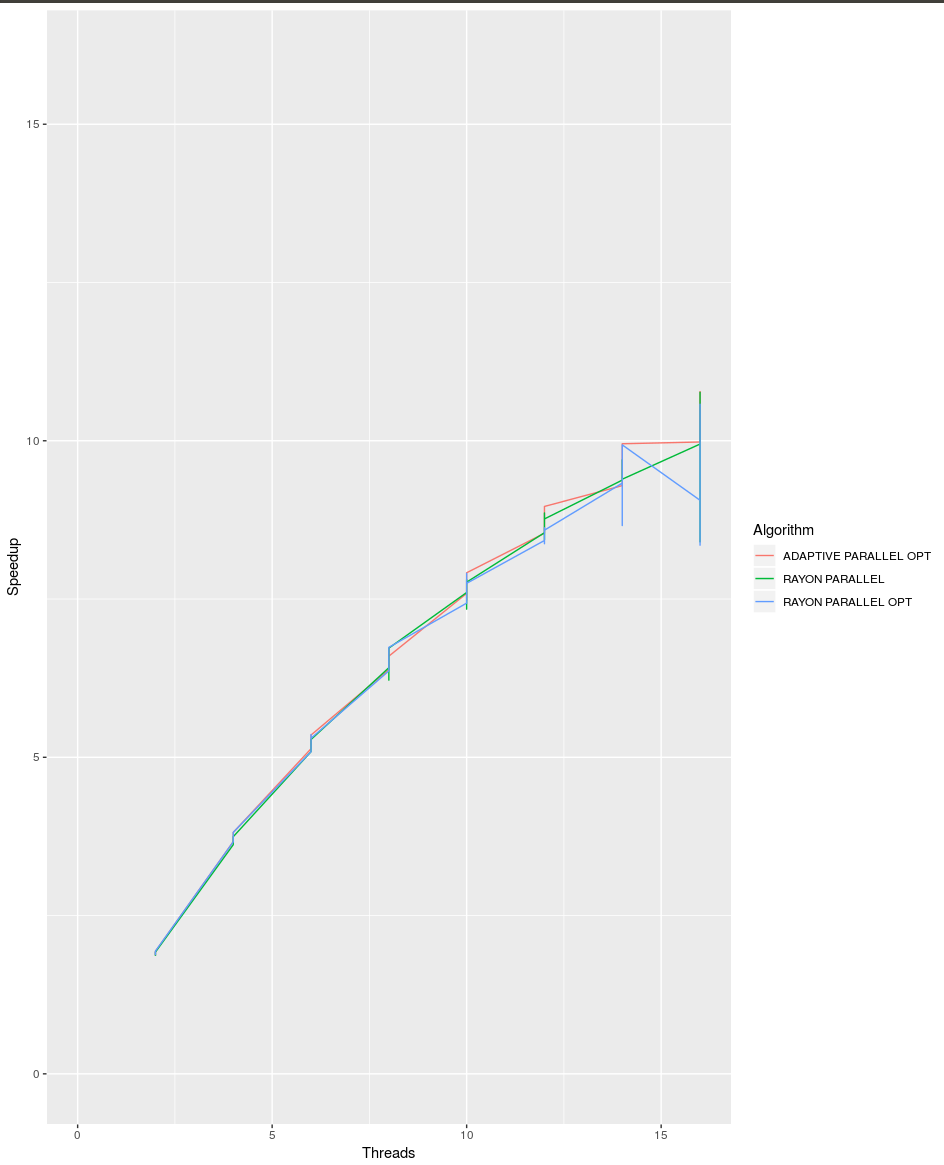
\includegraphics[scale=0.6]{Pictures/speedups.png}
	\rule{40em}{0.5pt}
    \caption[Optimization]{Speedup curves for the various parallel algorithms}
	\label{fig:speedups}
\end{figure}
The speedups were obtained as shown in Figure \ref{fig:speedups}. Here, it is important to note that the Adaptive API is undergoing some changes, hence the \emph{"Adaptive Parallel Opt"} algorithm actually uses the Rayon API for the $3^{rd}$ level of parallelization. Therefore, the speedups are quite similar for the algorithms.
%----------------------------------------------------------------------------------------


%-------------------------------------------------------------------------------
%	THESIS CONTENT - APPENDICES
%-------------------------------------------------------------------------------

\addtocontents{toc}{\vspace{2em}} % Add a gap in the Contents, for aesthetics

\appendix % Cue to tell LaTeX that the following 'chapters' are Appendices

% Include the appendices of the thesis as separate files from the Appendices
% folder
% Uncomment the lines as you write the Appendices

\input{Appendices/AppendixA}
%\input{Appendices/AppendixB}
%\input{Appendices/AppendixC}

\addtocontents{toc}{\vspace{2em}} % Add a gap in the Contents, for aesthetics

\backmatter

%-------------------------------------------------------------------------------
%	BIBLIOGRAPHY
%-------------------------------------------------------------------------------

\label{Bibliography}

\lhead{\emph{Bibliography}} % Change the page header to say "Bibliography"

\printbibliography

\end{document}
